%%%%%%%%%%%%%%%%%%%%%%%%%%%%%%%%%%%%%%%%%
% Wenneker Assignment
% LaTeX Template
% Version 2.0 (12/1/2019)
%
% This template originates from:
% http://www.LaTeXTemplates.com
%
% Authors:
% Vel (vel@LaTeXTemplates.com)
% Frits Wenneker
%
% License:
% CC BY-NC-SA 3.0 (http://creativecommons.org/licenses/by-nc-sa/3.0/)
% 
%%%%%%%%%%%%%%%%%%%%%%%%%%%%%%%%%%%%%%%%%

%----------------------------------------------------------------------------------------
%	PACKAGES AND OTHER DOCUMENT CONFIGURATIONS
%----------------------------------------------------------------------------------------

\documentclass[11pt]{scrartcl} % Font size

%%%%%%%%%%%%%%%%%%%%%%%%%%%%%%%%%%%%%%%%%
% Wenneker Assignment
% Structure Specification File
% Version 2.0 (12/1/2019)
%
% This template originates from:
% http://www.LaTeXTemplates.com
%
% Authors:
% Vel (vel@LaTeXTemplates.com)
% Frits Wenneker
%
% License:
% CC BY-NC-SA 3.0 (http://creativecommons.org/licenses/by-nc-sa/3.0/)
% 
%%%%%%%%%%%%%%%%%%%%%%%%%%%%%%%%%%%%%%%%%

%----------------------------------------------------------------------------------------
%	PACKAGES AND OTHER DOCUMENT CONFIGURATIONS
%----------------------------------------------------------------------------------------

\usepackage{amsmath, amsfonts, amsthm} % Math packages

\usepackage{listings} % Code listings, with syntax highlighting

\usepackage[english]{babel} % English language hyphenation

\usepackage{graphicx} % Required for inserting images
\usepackage{caption}
\graphicspath{{Figures/}{./}} % Specifies where to look for included images (trailing slash required)

\usepackage{booktabs} % Required for better horizontal rules in tables

\numberwithin{equation}{section} % Number equations within sections (i.e. 1.1, 1.2, 2.1, 2.2 instead of 1, 2, 3, 4)
\numberwithin{figure}{section} % Number figures within sections (i.e. 1.1, 1.2, 2.1, 2.2 instead of 1, 2, 3, 4)
\numberwithin{table}{section} % Number tables within sections (i.e. 1.1, 1.2, 2.1, 2.2 instead of 1, 2, 3, 4)

\setlength\parindent{0pt} % Removes all indentation from paragraphs

\usepackage{enumitem} % Required for list customisation
\setlist{noitemsep} % No spacing between list items

%----------------------------------------------------------------------------------------
%	DOCUMENT MARGINS
%----------------------------------------------------------------------------------------

\usepackage{geometry} % Required for adjusting page dimensions and margins

\geometry{
	paper=a4paper, % Paper size, change to letterpaper for US letter size
	top=2.5cm, % Top margin
	bottom=3cm, % Bottom margin
	left=3cm, % Left margin
	right=3cm, % Right margin
	headheight=0.75cm, % Header height
	footskip=1.5cm, % Space from the bottom margin to the baseline of the footer
	headsep=0.75cm, % Space from the top margin to the baseline of the header
	%showframe, % Uncomment to show how the type block is set on the page
}

%----------------------------------------------------------------------------------------
%	FONTS
%----------------------------------------------------------------------------------------

\usepackage[utf8]{inputenc} % Required for inputting international characters
\usepackage[T1]{fontenc} % Use 8-bit encoding

\usepackage{fourier} % Use the Adobe Utopia font for the document

%\usepackage[framed,numbered,autolinebreaks,useliterate]{mcode}

%----------------------------------------------------------------------------------------
%	SECTION TITLES
%----------------------------------------------------------------------------------------

\usepackage{sectsty} % Allows customising section commands

\sectionfont{\normalfont\bfseries} % \section{} styling
\subsectionfont{\normalfont\bfseries} % \subsection{} styling
\subsubsectionfont{\normalfont\itshape} % \subsubsection{} styling
\paragraphfont{\normalfont\scshape} % \paragraph{} styling

%----------------------------------------------------------------------------------------
%	HEADERS AND FOOTERS
%----------------------------------------------------------------------------------------

\usepackage{scrlayer-scrpage} % Required for customising headers and footers

\ohead*{} % Right header
\ihead*{} % Left header
\chead*{} % Centre header

\ofoot*{} % Right footer
\ifoot*{} % Left footer
\cfoot*{\pagemark} % Centre footer

% MY PACKAGES
%\usepackage[framed,numbered,autolinebreaks,useliterate]{mcode}
\usepackage{listings}
\usepackage{float}
\usepackage{amsmath}
\usepackage{tikz}
\usetikzlibrary{shapes,arrows,positioning}
\usepackage{hyperref} % Include the file specifying the document structure and custom commands

%----------------------------------------------------------------------------------------
%	TITLE SECTION
%----------------------------------------------------------------------------------------

\title{	
	\normalfont\normalsize
	\textsc{Universität Würzburg}\\ % Your university, school and/or department name(s)
	\vspace{25pt} % Whitespace
	\rule{\linewidth}{0.5pt}\\ % Thin top horizontal rule
	\vspace{20pt} % Whitespace
	{\huge Übung 8}\\ % The assignment title
	{\Large Beobachter}\\
	\vspace{12pt} % Whitespace
	\rule{\linewidth}{2pt}\\ % Thick bottom horizontal rule
	\vspace{12pt} % Whitespace
}

\author{\LARGE Alexander Björk, Janis Kaltenthaler} % Your name

\date{\normalsize\today} % Today's date (\today) or a custom date

\begin{document}

\maketitle % Print the title

\tikzstyle{block} = [draw, fill=blue!20, rectangle, 
    minimum height=3em, minimum width=6em]
\tikzstyle{sum} = [draw, fill=blue!20, circle, node distance=1cm]
\tikzstyle{input} = [coordinate]
\tikzstyle{output} = [coordinate]
\tikzstyle{pinstyle} = [pin edge={to-,thin,black}]
\newcommand{\inte}{$\displaystyle \int$}

\section*{Aufgabe 8-1. Beobachterentwurf (3 Punkte)}
\subsection*{a)}
Zu prüfen ist ob die Regelstrecke vollständig steuerbar und vollständig beobachtbar ist:
\subsubsection*{Steuerbarkeit}
\begin{align*}
	S_S&=\begin{bmatrix}b&Ab \end{bmatrix}=\begin{bmatrix}0&-0.5\\0.5&-1 \end{bmatrix}\\
	\text{det}\hspace{3pt}S_S&=0.25\neq0
\end{align*}
Die Regelstrecke ist vollständig Steuerbar.
\subsubsection*{Beobachtbarkeit}
\begin{align*}
	S_B&=\begin{bmatrix}C\\CA \end{bmatrix}=\begin{bmatrix}0&1\\1&-2 \end{bmatrix}\\
	\text{det}\hspace{3pt}S_B&=-1\neq0
\end{align*}
Die Regelstrecke ist vollsträndig beobachtbar.
\subsection*{b)}
Aufgrund der Strucktur des gegebenen Zustandsraummodells wissen wir dass dieses in der Beobachtungsnormalform vorliegt.\\
Die geforderten Eigenwerte des Beobachtermodells sind mit $\lambda_{B1}=-4$ und $\lambda_{B2}=-3$ gegeben. Daraus ergibt sich folgendes charakteristisches Polynom:
\begin{align*}
	p(\lambda_B)=\lambda^2+\underbrace{7}_{a_{B1}}\cdot\lambda+\underbrace{12}_{a_{B_0}}
\end{align*}
Die Koeffizienten $a_0=1$ und $a_1=2$ des charakteristischen Polynomes der Regelstrecke erhalten wird durch Ablesen aus dem gegebenen Zustandsraummodells.\\
Wie folgt kann nun die Beobachterrückführung berechnet werden:
\begin{align*}
	l^T=\begin{bmatrix}a_{B0}&a_{B1}\end{bmatrix}-\begin{bmatrix}a_{0}&a_{1}\end{bmatrix}=\begin{bmatrix}11&5\end{bmatrix}
\end{align*}

%Der Luenbergerbeobachter für das gegebene System hat nun die folgende Form:
%\begin{align*}
%	\dot{\hat{x}}(t)&=(A-lc^t)\hat{x}(t)+bu(t)+ly(t)\\
%	\dot{\hat{x}}(t)&=\begin{bmatrix}0&-12\\1&-7\end{bmatrix}\hat{x}(t)+\begin{bmatrix}0\\0.5\end{bmatrix}u(t)+\begin{bmatrix}11\\5\end{bmatrix}y(t)
%\end{align*}
Das Zustandsraummodell der Regelstrecke und des Beobachters erhält man wie folgt:
\begin{align*}
	\dot{\tilde{x}}(t)&=\begin{bmatrix}\dot{x}(t)\\\dot{\hat{x}}(t)\end{bmatrix}=\begin{bmatrix}A&0\\lc^T&A-lc^T\end{bmatrix}\cdot\begin{bmatrix}x(t)\\\hat{x}(t)\end{bmatrix}+\begin{bmatrix}B&E\\B&0\end{bmatrix}\cdot \begin{bmatrix}u(t)\\d(t)\end{bmatrix}\\
	y(t)&=\begin{bmatrix}C&0\end{bmatrix}\cdot\begin{bmatrix}x(t)\\\hat{x}(t)\end{bmatrix}\\\\
	\dot{\tilde{x}}(t)&=\begin{bmatrix}\dot{x}(t)\\\dot{\hat{x}}(t)\end{bmatrix}=\begin{bmatrix}0&-1&0&0\\1&-2&0&0\\0&11&0&-12\\0&5&1&-7\end{bmatrix}\cdot\begin{bmatrix}x(t)\\\hat{x}(t)\end{bmatrix}+\begin{bmatrix}0&0\\0.5&1\\0&0\\0.5&0\end{bmatrix}\cdot \begin{bmatrix}u(t)\\d(t)\end{bmatrix}\\
	y(t)&=\begin{bmatrix}0&1&0&0\end{bmatrix}\cdot\begin{bmatrix}x(t)\\\hat{x}(t)\end{bmatrix}
\end{align*}
\subsection*{c)}
\begin{figure}[H]
\centering
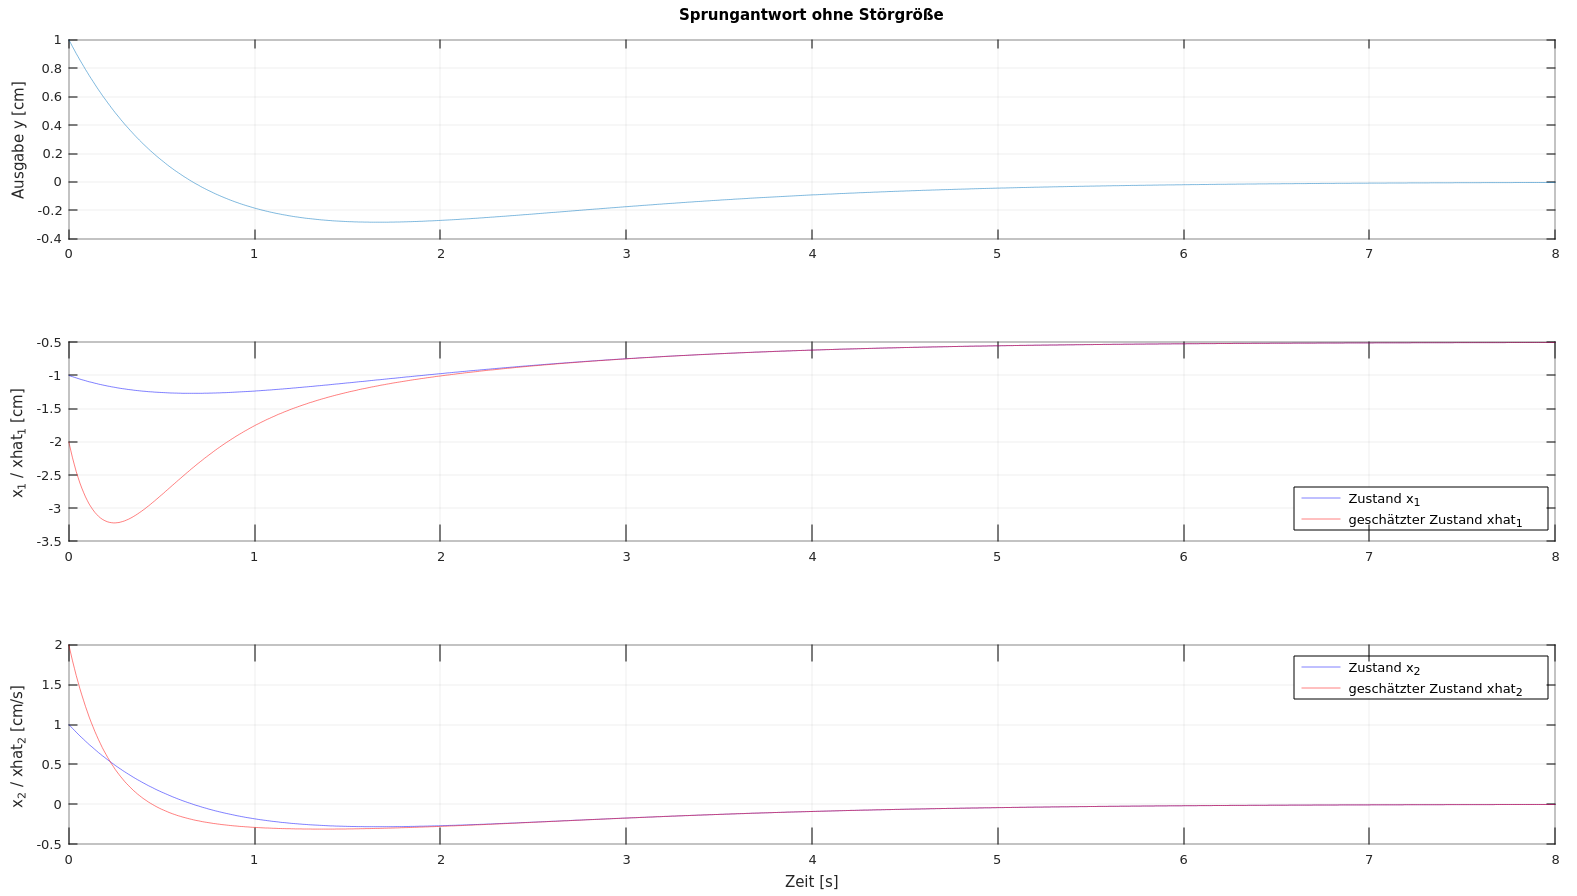
\includegraphics[width=\textwidth]{ohneStoergroesse.png}
\captionsetup{labelformat=empty}
\caption{Abb. 8-1.1: Sprungantwort ohne Störgröße.}
\end{figure}
Etwa zum Zeitpunkt $t=2s$ stimmt der geschätzte Zustand mit dem tatsächlichen Zustand überein.

\subsection*{d)}
\begin{figure}[H]
\centering
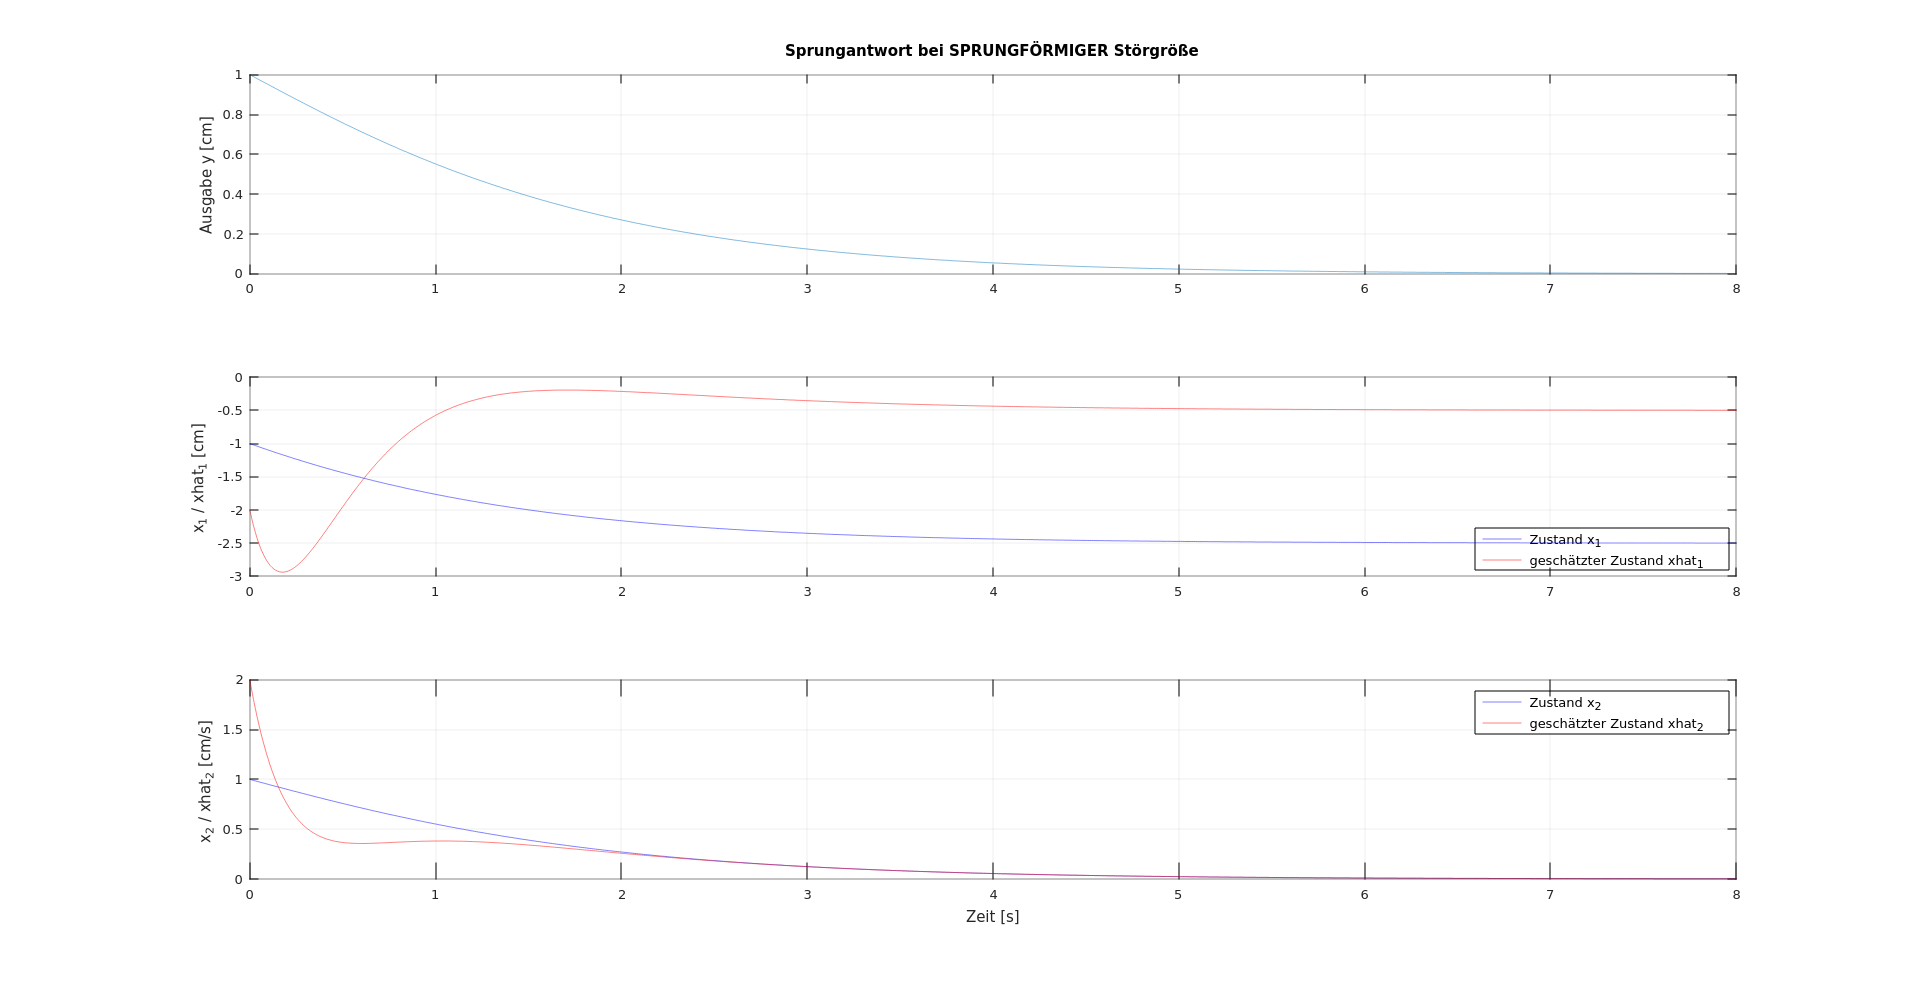
\includegraphics[width=\textwidth]{sprungfoermigeStoergroesse.png}
\captionsetup{labelformat=empty}
\caption{Abb. 8-1.2: Sprungantwort mit sprungförmiger Störgröße.}
\end{figure}

\begin{figure}[H]
\centering
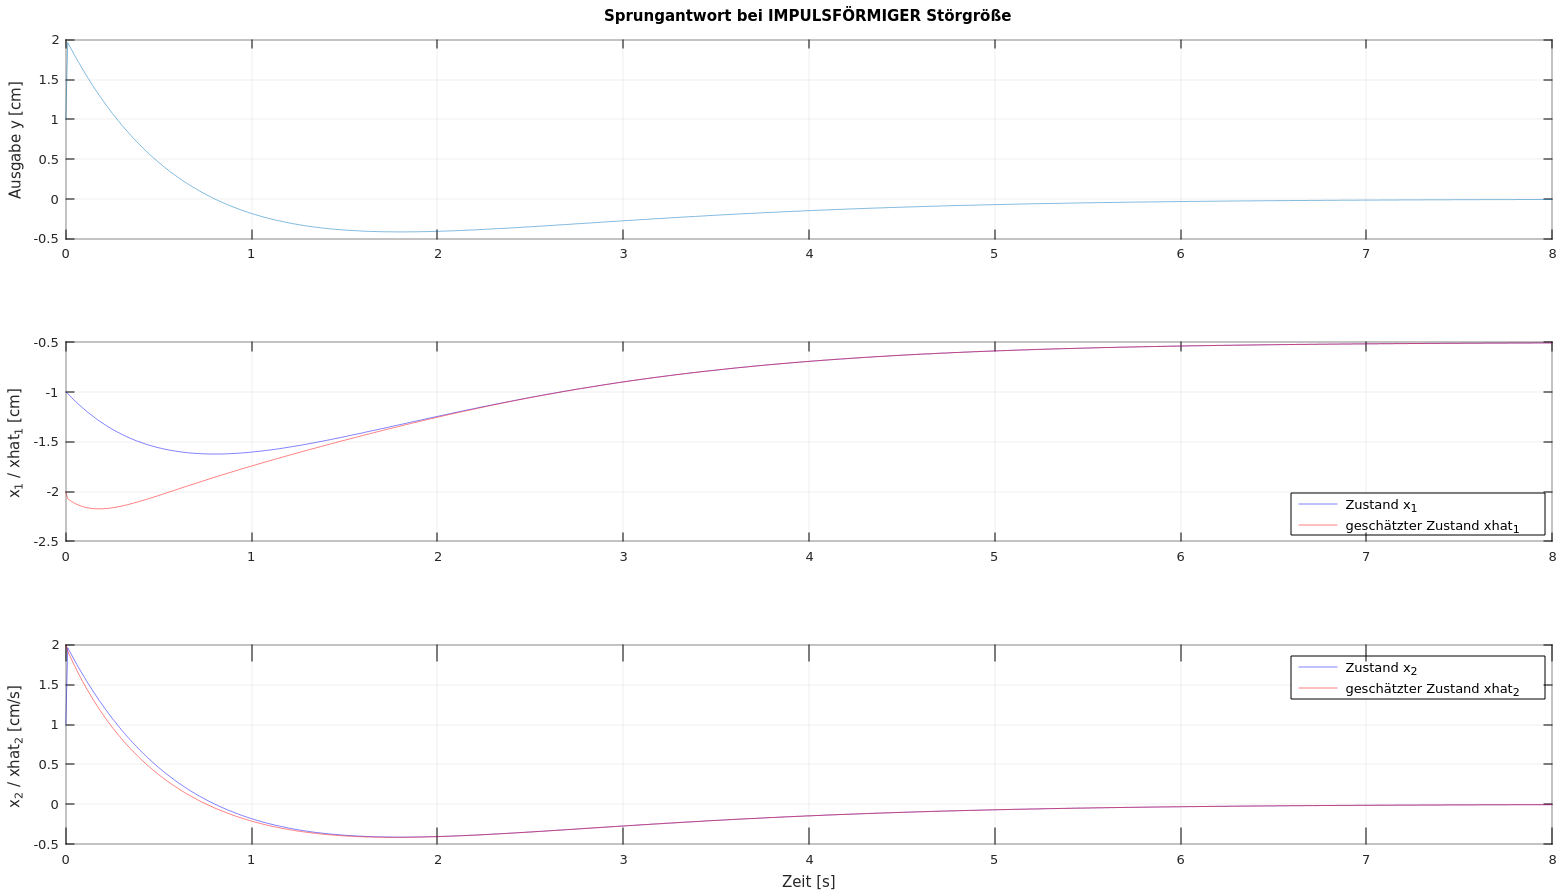
\includegraphics[width=\textwidth]{impulsfoermigeStoergroesse.png}
\captionsetup{labelformat=empty}
\caption{Abb. 8-1.3: Sprungantwort mit impulsförmiger Störgröße.}
\end{figure}

\begin{figure}[H]
\centering
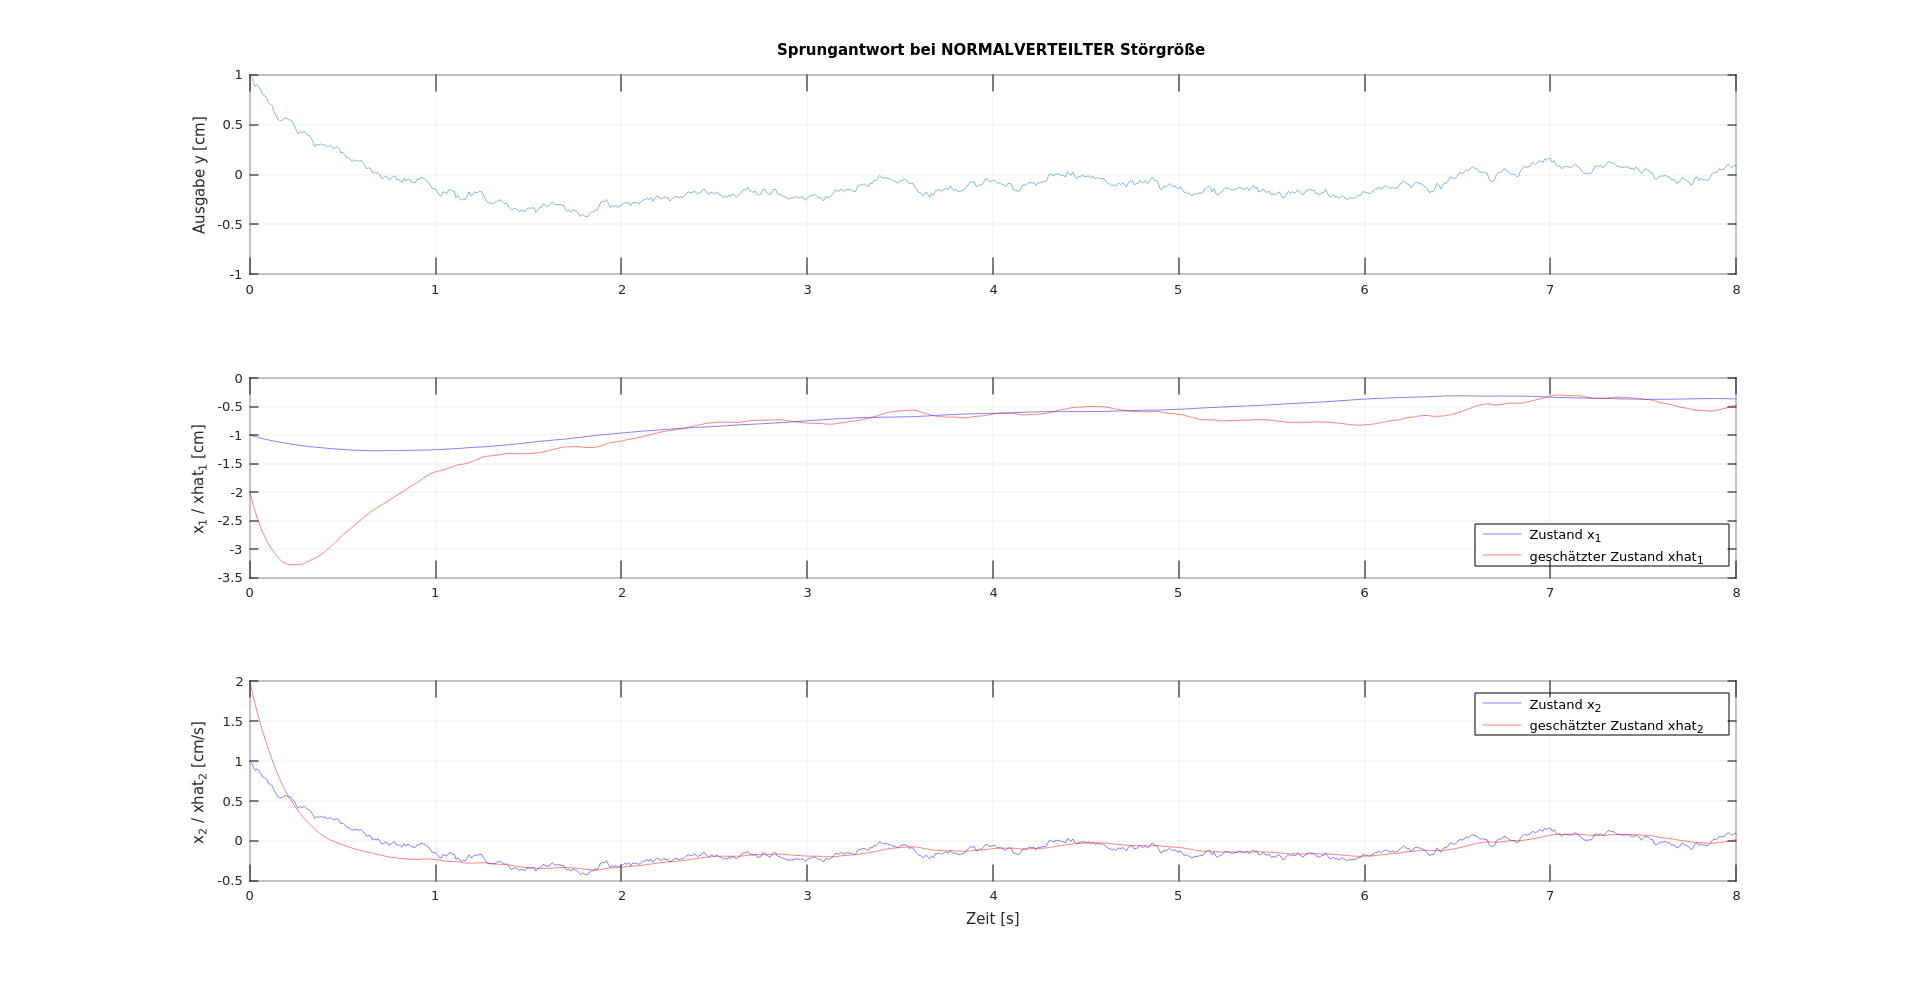
\includegraphics[width=\textwidth]{normalverteilteStoergroesse.png}
\captionsetup{labelformat=empty}
\caption{Abb. 8-1.4: Sprungantwort mit normalverteilter Störgröße.}
\end{figure}

Wirkt eine sprungförmige Störgröße auf die Regelstrecke, so bleibt eine stetige Abweichung zwischen dem geschätzten Zustand der ersten Zustandsvariable und dem tatsächlichen Zustand.\\
Wirkt eine normalverteilte oder impulsförmige Störgröße auf die Regelstrecke, so nähert sich sich der geschätzte Zustand dem tatsächlichen Zustand an.


\section*{Aufgabe 8-2. Beobachterentwurf mit Zustandsrückführung (3 Punkte)}
\subsection*{a)}
Die vollständige Steuerbarkeit und vollständige Beobachtbarkeit wurde mit Matlab geprüft.
\subsection*{b)}
Die Eigenwerte des Beobachters wurden mit $\lambda_{B1}=-9$ und $\lambda_{B2}=-12$ festgelegt.\\
Mithilfe von Matlab wurde das resultierende Zustandsraummodell des geschlossenen Regelkreises mit Beobachter berechnet:
\begin{align*}
	\dot{\tilde{x}}(t)&=\begin{bmatrix}\dot{x}(t)\\\dot{\hat{x}}(t)\end{bmatrix}=\begin{bmatrix}0&1&0&0\\-1&1&-11&-8\\22&0&-22&1\\129&0&-141&-7\end{bmatrix}\cdot\begin{bmatrix}x(t)\\\hat{x}(t)\end{bmatrix}+\begin{bmatrix}0\\12\\0\\12\end{bmatrix}\cdot u(t)\\
	y(t)&=\begin{bmatrix}0&1&0&0\end{bmatrix}\cdot\begin{bmatrix}x(t)\\\hat{x}(t)\end{bmatrix}
\end{align*}
\subsection*{c)}
Für die Simulation wurde eine sprungförmige Stellgröße genutzt. Die Anfangszustände wurden wie folgt gesetzt:
\begin{align*}
	x_0(t)=\begin{bmatrix}-1\\1\end{bmatrix},\hspace{10pt}\hat{x}_0(t)=\begin{bmatrix}-2\\2\end{bmatrix}
\end{align*}
\begin{figure}[H]
\centering
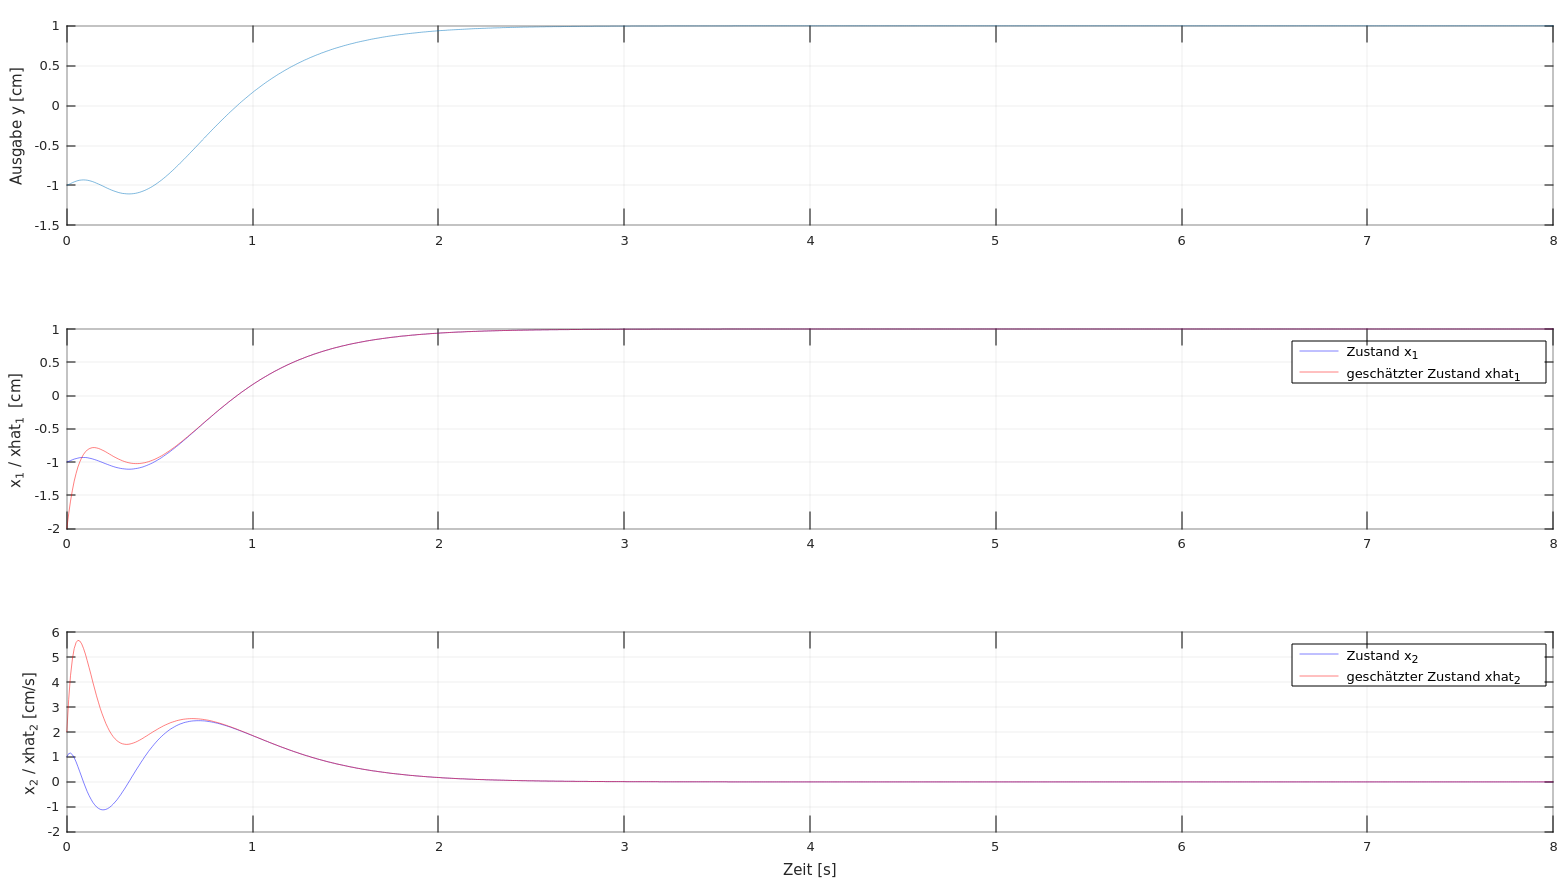
\includegraphics[width=\textwidth]{beobachterentwurfMitZustandsrueckfuehrung.png}
\captionsetup{labelformat=empty}
\caption{Abb. 8-2.1: Sprungantwort.}
\end{figure}

\end{document}
